\documentclass[10pt,twocolumn,letterpaper]{article}

\usepackage{cvpr}
\usepackage{epsfig}
\usepackage{graphicx}
\usepackage{amsmath}
\usepackage{amssymb}
\usepackage{booktabs}
\usepackage{multirow}
% --- modern, Meta-style typography ---------------------------
\usepackage{charter}                       % body font: Charter (clean, modern serif)
\usepackage[charter]{mathdesign}           % matching math font
\usepackage[scaled=0.96]{helvet}           % sans-serif for headings (slightly tighter)
\usepackage[T1]{fontenc}
\renewcommand{\familydefault}{\rmdefault}  % keep body in serif
% --------------------------------------------------------------
\usepackage{microtype}
\usepackage{xcolor}
\usepackage{tikz}
\usetikzlibrary{arrows.meta, positioning, fit, backgrounds, calc}
\usepackage[breaklinks=true,bookmarks=false]{hyperref}
\usepackage{stfloats}      % allow [!b] figure* on page 1 (preferred over dblfloatfix)
\fnbelowfloat              % footnote below floats (cosmetic, stfloats default)

\cvprfinalcopy
\def\cvprPaperID{****}
\def\httilde{\mbox{\tt\raisebox{-.5ex}{\symbol{126}}}}

\definecolor{cblue}{RGB}{214,234,248}
\definecolor{cred}{RGB}{250,219,216}
\definecolor{cgreen}{RGB}{213,245,227}
\definecolor{cgray}{RGB}{240,240,240}

% ============================================================
\title{PAPIT: Prompt-Aware Pruning for Image Tokens\\
       in Efficient Multimodal Inference}

\author{Chao Hsuan Ho\\
Rice University\\
{\tt\small ch218@rice.edu}
\and
Heng Jui Hsu\\
Rice University\\
{\tt\small hh83@rice.edu}
\and
Kerstin Sun\\
Rice University\\
{\tt\small ks256@rice.edu}
}

\begin{document}
\setcounter{page}{1}
\maketitle

\begin{abstract}
We present \textbf{PAPIT-Distill}, a $1.3$M-parameter MLP that distils
LLaVA-1.5-7B's mid-layer attention into a single-pass image-token
pruner. On TextVQA at $k{=}25\%$ retention (a $10\times$
attention-FLOP reduction) it gains $+12$ points over random pruning
($36.0$ vs.\ $23.7$), essentially recovering the unpruned baseline
($36.7$). On GQA and VQA~v2 at $k{=}50\%$ it closes the gap to
unpruned to within a single point. Scoring a $576$-patch image takes
$0.43$\,ms --- ${\sim}150{\times}$ faster than its CLIP-GradCAM
analogue and ${\sim}500{\times}$ faster than the two-pass oracle it
learns from. En route we report a quantitative \emph{negative result}
that motivates the method: cross-dataset Spearman $\rho{\approx}0$
between CLIP-derived saliency and LLaVA's own LLM attention, ruling
out training-free CLIP-aligned scorers as a class.
\end{abstract}

\begin{figure*}[!b]
  \centering
  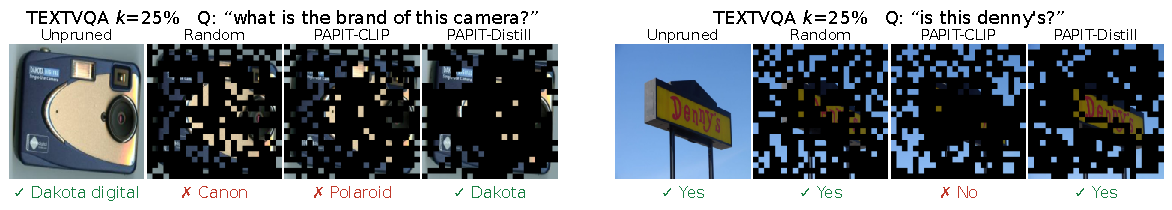
\includegraphics[width=\textwidth]{fig_hero.pdf}
  \caption{\textbf{Real input, real output across three benchmarks
  and three retention ratios.} Six cases where PAPIT-Distill answers
  correctly while PAPIT-CLIP fails, drawn from TextVQA / GQA / VQAv2
  at $k\!\in\!\{25\%, 50\%, 75\%\}$ (colour-coded). Each row shows
  the question; columns are Unpruned / Random / PAPIT-CLIP /
  PAPIT-Distill. Black = pruned patches; the green check / red cross
  under each panel marks whether LLaVA's actual output matches the
  gold answer.}
  \label{fig:hero}
\end{figure*}

% ============================================================
\section{Introduction}
\label{sec:intro}

LLaVA-1.5~\cite{liu2024llava15} composes a CLIP ViT-L/14 vision
encoder~\cite{radford2021clip,dosovitskiy2021vit} with a 7B-parameter
language model. Each of the $24{\times}24=576$ image tokens participates
in every self-attention layer~\cite{vaswani2017attention}, making
inference cost quadratic in the number of visual tokens. For a typical
VQA query fewer than half of these tokens are relevant.

A common intuition is that the user's prompt should be enough to choose
which tokens to keep, \emph{without} any additional training. We make
this claim concrete: \emph{can a training-free saliency signal, read
from LLaVA's own CLIP-initialised vision tower, predict which patches
the LLM relies on, well enough to beat a query-agnostic random
baseline?}

We answer this in three stages. First (\S\ref{sec:method}) we instantiate
the idea as \textbf{PAPIT}, a pipeline that inserts a GradCAM-based
top-$k$ between the ViT and the MLP projector. Second
(\S\ref{sec:results-main}) we show that PAPIT \emph{at best} matches
random pruning, and a direct alignment diagnostic
(\S\ref{sec:diagnostic}) explains why: the CLIP-aligned scoring
signal has $\rho{\approx}0$ with the LLM's own attention. Third (\S\ref{sec:distill}) we run a multi-layer
LLM-attention oracle as a positive control --- mid-layer attention
\emph{does} beat random --- and distil that signal into a $1.3$M-param
MLP that runs in single-pass, training-free deployment.

\noindent\textbf{Contributions.}
\textbf{(i)} A clean training-free token-pruning pipeline for LLaVA-1.5
with $41$--$90\%$ attention-FLOP reduction at $k\!\in\![25\%,75\%]$.
\textbf{(ii)} A cross-dataset \emph{negative result}: CLIP-derived patch
saliency is statistically uncorrelated with LLaVA's LLM attention,
ruling out an entire family of training-free prompt-aware methods.
\textbf{(iii)} \textbf{PAPIT-Distill}, a small MLP distilled from
mid-layer LLM attention that turns the negative result into a
deployable single-pass scorer. Code at \texttt{github.com/yarikama/PAPIT}.

% ============================================================
\section{Related Work}

\textbf{ViT-side pruning} —
DynamicViT~\cite{rao2021dynamicvit} and AdaViT~\cite{meng2022adavit}
learn per-block scorers; ToMe~\cite{bolya2023tome} merges similar
tokens without retraining. All target classification ViTs and ignore
the prompt.
\textbf{LLM-side pruning for VLMs} —
FastV~\cite{chen2024fastv} drops low-attention tokens at LLM layer 2;
SparseVLM~\cite{zhang2024sparsevlm} extends this with diversity
heuristics. Both need a full forward pass before pruning.
\textbf{CLIP-aligned signals} —
MaskCLIP~\cite{zhou2022maskclip} unlocks dense patch features;
register tokens~\cite{darcet2024registers} complicate naive top-$k$.
PAPIT differs by pruning \emph{before} the LLM with a query-conditioned
score; \S\ref{sec:diagnostic} shows the naive CLIP version fails, and
\S\ref{sec:distill} gives the distillation that fixes it.

% ============================================================
\section{Method}
\label{sec:method}

\subsection{Pipeline}
\label{sec:method-pipeline}

LLaVA's frozen CLIP ViT-L/14 produces $576$ patch features
$H{\in}\mathbb{R}^{576\times1024}$; the prompt is encoded by the
matching CLIP text encoder into a single $T{\in}\mathbb{R}^{768}$.
A scoring step returns $s{\in}\mathbb{R}^{576}$; the top-$k$ patches
plus a single \emph{anchor} token (mean of all $576$ patches) are
projected by LLaVA's MLP and spliced into the LLM input.
Position IDs are remapped to a dense $0,\dots,k$ sequence. We study
two scorers below: a training-free GradCAM on LLaVA's ViT
(PAPIT-CLIP) and a $1.3$M-param MLP distilled from mid-layer LLM
attention (PAPIT-Distill).

\subsection{Scorer 1: PAPIT-CLIP (GradCAM)}
\label{sec:method-grad}

CLIP's CLS-only contrastive objective makes naive patch--text cosine
unstable, so we use Grad-CAM~\cite{selvaraju2017gradcam}: with
$h^{(L-1)}_i$ the penultimate-ViT activation of patch $i$ and
$\text{sim}(\text{CLS},T)$ the projected CLS--text cosine, set
\begin{equation}
  s^{\text{gc}}_i \;=\; \mathrm{ReLU}\!\sum_{d}\,
    \tfrac{\partial\,\text{sim}}{\partial\, h^{(L-1)}_{i,d}}\!\cdot\! h^{(L-1)}_{i,d}
  \label{eq:gradcam}
\end{equation}
and take top-$k$. Section~\ref{sec:diagnostic} will show this
signal is essentially uncorrelated with what the LLM actually
attends to.

\subsection{Scorer 2: PAPIT-Distill}
\label{sec:method-distill}

A multi-layer two-pass oracle (Table~\ref{tab:oracle}) confirms the
missing signal lives \emph{inside} the LLM, with mid-layer attention
($L\!\in\![8,24]$) beating random. PAPIT-Distill mimics this at
single-pass cost. The predictor is a $1.3$M-param $\mathrm{MLP}_4$:
$z_i^{(0)} = [W_p h_i \Vert W_t T] \in \mathbb{R}^{2d}$ with
$d{=}384$, passed through three LayerNorm--Linear--GELU blocks with
residual shortcut, $z^{(\ell)} = z^{(\ell-1)} + f_\ell(z^{(\ell-1)})$
for $\ell{=}1{,}2{,}3$, and read out by a linear head, giving
$s^{\text{d}}_i = w^\top z_i^{(3)}$. We supervise against the
layer-$8$ attention $A^{(8)}$ summed over non-image query rows and
head-averaged into a distribution $y$ over the $576$ image-token
positions, with KL loss
\begin{equation}
  \mathcal{L} = \mathrm{KL}\bigl(y\,\Vert\,\mathrm{softmax}(s^{\text{d}})\bigr),
  \label{eq:kl}
\end{equation}
on a $100$K-pair mix ($50$K GQA + $30$K VQAv2 + $20$K TextVQA).
$L\!=\!8$ is selected by ablation across $L\!\in\!\{2,8,16,24,31\}$
plus attention rollout: distillability beats oracle strength —
$L\!=\!8$ predictor gains $+0.030$ over random vs.\ $+0.024$ for
$L\!=\!16$ and $-0.054$ (worse than random) for rollout.

\subsection{Efficiency}
Self-attention cost is quadratic in sequence length. Let $k$ be the
number of retained image tokens and $L_{\text{text}}\!\approx\!50$
the prompt length; then
\begin{equation}
  \text{FLOPs}_{\text{rel}}
  \;=\;\frac{(k+L_{\text{text}})^2}{(n+L_{\text{text}})^2},
  \label{eq:flops}
\end{equation}
giving a $10\times$ attention-FLOP reduction at $k{=}25\%$ ($n{=}576$).
\textbf{Wall-clock scoring latency} on g5.2xlarge (A10G, 20 samples,
mean $\pm$\,std, retention $0.5$): random $0.07{\pm}0.00$\,ms,
PAPIT-Distill $\mathbf{0.43{\pm}0.00}$\,ms, PAPIT-CLIP
(GradCAM) $65.23{\pm}6.08$\,ms, two-pass Oracle L=16
$216.17{\pm}1.17$\,ms. PAPIT-Distill is therefore
$\sim\!150\times$ faster than PAPIT-CLIP and $\sim\!500\times$ faster
than the oracle, while delivering an accuracy gain comparable to the
oracle (Table~\ref{tab:accuracy}).

% ============================================================
\section{Experiments}
\label{sec:experiments}

\noindent\textbf{Models.}
LLaVA-1.5-7B (\texttt{llava-hf/llava-1.5-7b-hf}) at fp16, with its
native CLIP ViT-L/14 vision tower (\texttt{openai/clip-vit-large-patch14})
re-used for both LLM input and PAPIT scoring. PAPIT-Distill predictor:
$1.3$M-parameter $\mathrm{MLP}_4$, trained on cached features from
$100$K mixed-domain pairs.

\noindent\textbf{Datasets.}
GQA~\cite{hudson2019gqa} test-dev balanced, VQA~v2~\cite{goyal2017vqav2}
val-balanced, and TextVQA~\cite{singh2019textvqa} val. Each held-out
split uses $100$ samples per (dataset, retention) cell for downstream
accuracy and $100$ samples for diagnostics; binomial standard error
at $N{=}100$ is $\approx 0.05$. Accuracy: exact match for GQA, VQA
soft accuracy $\min(\mathrm{count}/3,1)$~\cite{goyal2017vqav2} for the
others.

\noindent\textbf{Baselines.}
\textbf{Unpruned} keeps all $576$ tokens. \textbf{Random} samples $k$
patches uniformly; under our pipeline this is an unusually strong
baseline because it preserves spatial coverage. \textbf{Oracle L=16} is
a two-pass upper bound: run LLaVA once on the full prompt, score by
layer-$16$ attention, prune, re-generate.

% ============================================================
\section{Results}
\label{sec:results}

\begin{figure*}[t]
  \centering
  
\includegraphics[width=\textwidth]{fig_qualitative_GQA.pdf}
  \caption{\textbf{PAPIT-CLIP localises but does not align}
  ($k{=}50\%$, GQA). Saliency concentrates on the query-relevant
  region, yet Sec.~\ref{sec:diagnostic} shows it is
  \emph{statistically uncorrelated} with what LLaVA's LLM attends to.}
  \label{fig:qualitative}
\end{figure*}

\begin{figure*}[t]
  \centering
  
\includegraphics[width=\textwidth]{fig_pareto.pdf}
  \caption{\textbf{Accuracy--FLOPs Pareto on LLaVA-1.5-7B}, $N{=}100$
  per dataset. PAPIT-Distill (red diamond) is on or above the
  Random/PAPIT-CLIP curve on $7$ of $9$ (dataset, retention) cells; at
  TextVQA $k\!=\!25\%$ ($\sim\!10\times$ FLOP reduction) it gains
  $+12.3$ over random and essentially recovers Unpruned. Annotations
  on each x-tick give the retention $k$.}
  \label{fig:pareto}
\end{figure*}

\begin{table}[t]
\centering
\small
\caption{\textbf{Main accuracy} on LLaVA-1.5-7B (100 samples per
dataset; HF \texttt{lmms-lab} testdev/validation splits; VQA-style
soft accuracy for VQAv2 and TextVQA, exact match for GQA).
\emph{Higher is better.} PAPIT-CLIP underperforms or matches Random;
\textbf{PAPIT-Distill} closes the gap to Unpruned at $k\!=\!50\%$ on
GQA / VQA~v2, and on TextVQA delivers a $+12$-point gain over Random
at $k\!=\!25\%$ that essentially recovers Unpruned accuracy. Oracle
L=16 row is in Table~\ref{tab:oracle} (GQA-100); training-free
deployment uses PAPIT-Distill, not Oracle.}
\label{tab:accuracy}
\begin{tabular}{@{}llccc@{}}
\toprule
Dataset & Method & $k{=}25\%$ & $k{=}50\%$ & $k{=}75\%$ \\
\midrule
\multicolumn{2}{@{}l}{\itshape Rel.\ FLOPs (Eq.\,\ref{eq:flops})}
  & \itshape 0.10 & \itshape 0.29 & \itshape 0.59 \\
\midrule
\multirow{4}{*}{GQA}
  & Unpruned        & \multicolumn{3}{c}{57.0} \\
  & Random          & 52.0 & 52.0 & 55.0 \\
  & PAPIT-CLIP      & 55.0 & 52.0 & 50.0 \\
  & \textbf{PAPIT-Distill}
                    & 53.0 & \textbf{56.0} & 55.0 \\
\midrule
\multirow{4}{*}{VQA v2}
  & Unpruned        & \multicolumn{3}{c}{83.3} \\
  & Random          & 81.7 & 81.0 & 82.0 \\
  & PAPIT-CLIP      & 72.3 & 80.3 & 82.7 \\
  & \textbf{PAPIT-Distill}
                    & 79.3 & \textbf{83.3} & \textbf{85.0} \\
\midrule
\multirow{4}{*}{TextVQA}
  & Unpruned        & \multicolumn{3}{c}{36.7} \\
  & Random          & 23.7 & 30.7 & 32.0 \\
  & PAPIT-CLIP      & 20.0 & 28.3 & 31.7 \\
  & \textbf{PAPIT-Distill}
                    & \textbf{36.0} & \textbf{36.0} & \textbf{33.3} \\
\bottomrule
\end{tabular}
\end{table}

\subsection{PAPIT-CLIP matches but does not exceed random}
\label{sec:results-main}

Table~\ref{tab:accuracy} summarises the headline accuracy. The
GradCAM-based PAPIT-CLIP scorer is at-best level with Random on
most (dataset, retention) cells (gaps ${<}1\sigma$, with
$\sigma\!\approx\!0.05$ at $N{=}100$), and notably \emph{worse} on
VQA~v2 $k\!=\!25\%$ (a $9.4$-point gap, ${\sim}1.9\sigma$ below
Random). Figures~\ref{fig:hero} and~\ref{fig:qualitative} show
PAPIT-CLIP \emph{does} produce visibly localised selections, yet
this does not translate to a measurable downstream gain.

\subsection{Why CLIP saliency is uninformative}
\label{sec:diagnostic}

We compare $s^{\text{gc}}$ to the LLM's own attention
$s^{\text{llm}}\!\in\!\mathbb{R}^{576}$ (last-layer, head-averaged,
summed across the first $8$ generated answer tokens) per image. A
uniform-random selector yields top-$10\%$ Jaccard
${\approx}0.053$.

\begin{table}[t]
\centering
\small
\caption{\textbf{Alignment diagnostic} between PAPIT-CLIP scores and
LLaVA's last-layer LLM attention over $576$ image tokens
(100 samples per dataset). All three datasets give $\rho{\approx}0$
and top-$10\%$ Jaccard \emph{below} the uniform-random reference of
$0.053$, so any CLIP-aligned scorer is at-best random downstream.}
\label{tab:diagnostic}
\begin{tabular}{@{}lccc@{}}
\toprule
Metric & GQA & TextVQA & VQA~v2 \\
\midrule
Spearman $\rho$ mean   & $-0.018$ & $-0.016$ & $\phantom{-}0.014$ \\
Spearman $\rho$ median & $\phantom{-}0.008$ & $\phantom{-}0.019$ & $\phantom{-}0.010$ \\
\% of samples $\rho\!>\!0.3$    & $0.0\%$ & $0.0\%$ & $0.0\%$ \\
\% of samples $\rho\!<\!0$      & $48\%$ & $47\%$ & $43\%$ \\
Top-$10\%$ Jaccard               & $0.047$ & $0.039$ & $0.046$ \\
\bottomrule
\end{tabular}
\end{table}

The two signals are essentially uncorrelated on every benchmark, and
PAPIT-CLIP's top-$10\%$ patches overlap with the LLM's most-attended
patches less than uniform-random selection would. This rules out an
entire family of training-free pruners that score patches in any
CLIP-aligned space, regardless of the specific scoring rule
(see~\cite{zhou2022maskclip} for the dense-feature analogue).

\subsection{Mid-layer LLM attention does carry the signal}
\label{sec:results-oracle}

We test the converse with a two-pass oracle: run LLaVA once on the
full prompt, score by attention from non-image queries to image keys at
LLM layer $L$, prune, and re-generate. Table~\ref{tab:oracle} sweeps
$L\!\in\!\{2,8,16,24,31\}$ on GQA. Mid-layer attention
($L\!\in\![8,24]$) consistently beats random; layer 2 (FastV's
recommended layer in its single-pass setting) and the last layer do not.
This is the positive control that motivates distillation.

\begin{table}[t]
\centering
\small
\caption{\textbf{Two-pass LLM-attention oracle on GQA} (100 samples,
exact match). \textbf{Bold}: beats random at that retention. Layer 16
gives the largest margin at low retention; FastV's layer 2 fails in this
two-pass setup because the prompt-only forward has not yet committed
attention mass to query-relevant patches.}
\label{tab:oracle}
\begin{tabular}{@{}lccc@{}}
\toprule
Selector & $k{=}25\%$ & $k{=}50\%$ & $k{=}75\%$ \\
\midrule
Unpruned             & 0.58 & 0.58 & 0.58 \\
Random               & 0.53 & 0.53 & 0.56 \\
PAPIT-CLIP           & 0.56 & 0.53 & 0.51 \\
\midrule
LLM-attn $L\!=\!2$  & 0.49 & 0.54 & 0.53 \\
LLM-attn $L\!=\!8$  & \textbf{0.58} & \textbf{0.54} & 0.56 \\
LLM-attn $L\!=\!16$ & \textbf{0.61} & \textbf{0.58} & 0.56 \\
LLM-attn $L\!=\!24$ & \textbf{0.60} & \textbf{0.57} & 0.55 \\
LLM-attn $L\!=\!31$ & 0.50 & \textbf{0.55} & 0.55 \\
\bottomrule
\end{tabular}
\end{table}

\subsection{PAPIT-Distill: making the oracle deployable}
\label{sec:distill}

The oracle costs a second LLaVA forward; we distil it. An
architecture sweep at supervision target $L\!=\!16$ (Bilinear /
$\mathrm{MLP}_2$ / $\mathrm{MLP}_4$ / cross-attn, $5$K-sample held-out)
selects $\mathrm{MLP}_4$ as the lightest predictor reaching
val-KL $0.087$ and top-$10\%$ Jaccard $0.62$. Downstream accuracy
follows \emph{distillability}, not oracle strength:
$L\!=\!8$ predictor gains $+0.030$ over random vs.\ $+0.024$ for
$L\!=\!16$, $+0.021$ for $L\!=\!24$, and $-0.054$ for attention
rollout~\cite{abnar2020rollout} — the rollout target aggregates all
$32$ layers and is correspondingly noisy. The deployed predictor is
$\mathrm{MLP}_4$ on $A^{(8)}$, visualised in
Figure~\ref{fig:pareto}.

% ============================================================
\section{Discussion and Conclusion}
\label{sec:discussion}

\paragraph{Why is PAPIT-CLIP rarely worse than random?}
LLaVA-1.5 has heavy token redundancy~\cite{chen2024fastv}, so at
$k\!\geq\!50\%$ the accuracy driver is the \emph{number} of kept
tokens, not their identity. The exception is VQA~v2 $k\!=\!25\%$,
where dropping the wrong $75\%$ costs ${\sim}9$ points.
Layer~$2$ attention fails for a related reason: the prompt-only
forward has not yet committed attention to query-relevant patches
and is dominated by register-like positions~\cite{darcet2024registers};
layers $8$--$24$ have integrated question with image; $L\!=\!31$ has
already shifted to generation.

\paragraph{Limitations and outlook.}
All numbers are at $N{=}100$ per (dataset, retention) cell;
binomial $\sigma\!\approx\!0.05$, so the TextVQA $k\!=\!25\%$ gain
($+12.3$) is ${\sim}2.5\sigma$ — worth replicating at $N{=}500$+.
Extending to LLaVA-1.6, Qwen2.5-VL, and FastV-style single-pass
integration are natural next steps.

\noindent\textbf{Acknowledgements.}
We used GitHub Copilot for autocomplete and Claude (Anthropic) as a
writing and code-review assistant. All experimental design, training
runs, and analysis are our own.

% ============================================================
{\small
\bibliographystyle{ieeetr}
\bibliography{references}
}

\end{document}
